\chapter{静电学}

\section{电场}

\paragraph*{库仑定律}
空间中一静止电荷$q$,一检验电荷$Q$,两者相距$\brcurs$,库伦定律指出两者间的库仑作用力
为
\begin{equation}
    \bm{F} = \frac{1}{4\pi\epsilon_0}\frac{qQ}{\rcurs^2} \hat{\bm{r}}
    \label{eq:Coulomb-law}
\end{equation}
其中,$\epsilon_0$为真空介电常数。在SI单位制中,力单位为${\rm N}$,距离单位为$\rm m$,
电荷单位为$\rm C$,故有
\begin{equation}
    \epsilon_0 = 8.85 \times 10^{-12} \frac{{\rm C}^2}{{\rm N}\cdot {\rm m^2}}
    \label{eq:permit-zero}
\end{equation}
间隔矢量$\hrcurs$表示沿$\brcurs = \bm{r} - \bm{r}^{\prime}$方向的单位矢量。

\paragraph*{电场}
有若干点电荷$\bm{q}_1$、$\bm{q}_2$、$\cdots$、$\bm{q}_n$,它们与检验电荷间距离分别为
$\brcurs_1$、$\brcurs_2$、$\cdots$、$\brcurs_n$,其对检验电荷都有力的作用,根据库仑
定律及力的合成规则,总的力为
\begin{equation*}
    \begin{aligned}
        \bm{F} &= \bm{F}_1 + \bm{F}_2 + \cdots + \bm{F}_n    \\
               &= \frac{1}{4\pi\epsilon_0}\left( 
                    \frac{q_1Q}{\rcurs_1}\hrcurs_1
                  + \frac{q_2Q}{\rcurs_2}\hrcurs_2
                  + \cdots
                  + \frac{q_nQ}{\rcurs_n}\hrcurs_n
               \right) \\
               &= \frac{Q}{4\pi\epsilon_0}\left( 
                    \frac{q_1}{\rcurs_1}\hrcurs_1
                  + \frac{q_2}{\rcurs_2}\hrcurs_2
                  + \cdots
                  + \frac{q_n}{\rcurs_n}\hrcurs_n
               \right) \\
               &= q\bm{E}
    \end{aligned}
\end{equation*}
产生电场的那些电荷称为源电荷,所在位置为源点,把
\begin{equation}
    \bm{E}(\bm{r}) = \frac{1}{4\pi\epsilon}
                     \sum_{i=1}^{n}\frac{q_i}{\rcurs_i^2}\hrcurs_i
    \label{eq:electric-field}
\end{equation}
称为源电荷的电场,电场单位为${\rm N/C} a$,$\bm{r}$是原点到场点的矢量间隔,如下图:
\begin{figure}[ht]
    \centering
    \setlength{\abovecaptionskip}{0.2cm}
    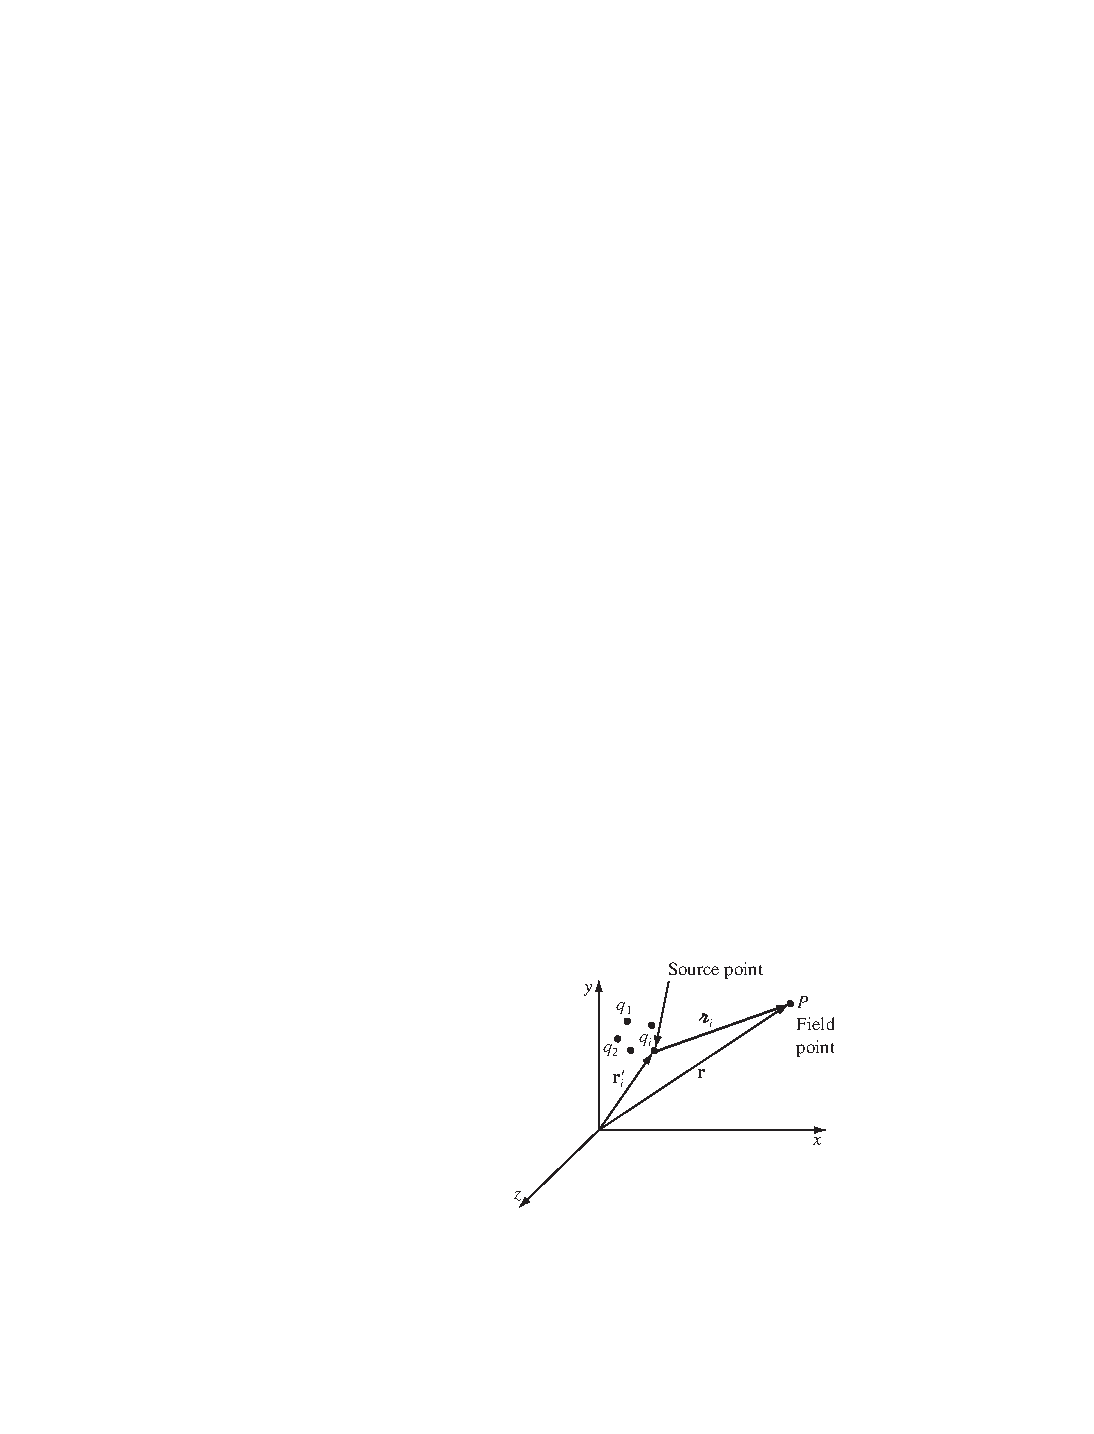
\includegraphics{./figure/electrodynamics/elec-filed-example.pdf}
    \caption{}
    \label{fig:elec-field}
\end{figure}

\begin{note}
    $\bm{E}(\bm{r})$为坐标$\bm{r}$的函数。
\end{note}

\uline{电场的物理解释}:电场表示单位电荷在场点处受到的力。

若电荷分布具有连续性,则将\ref{eq:electric-field}中的求和改为积分,就得到连续分布电荷
的电场
\begin{equation}
    \bm{E}(\bm{r}) = \frac{1}{4\pi\epsilon}\int\frac{1}{\rcurs^2}\hrcurs \,dq
    \label{eq:cont-elec-field}
\end{equation}

\section{静电场散度和旋度}

\paragraph*{电场强度通量}
电场强度是描述电场强弱的量,电场强度通量定义为
\begin{equation}
    \Phi_k = \int_{S} \bm{E} \cdot \, d\bm{a}
    \label{eq:elec-field-flux}
\end{equation}
这里$S$表示电场强度通过的表面,$\bm{a}$表示上面的一个矢量面元。

\paragraph*{高斯定理}
高斯定理的积分形式:

高斯定理的微分形式:


